% -*-latex-*-
%
%  The contents of this file are subject to the University of Utah Public
%  License (the "License"); you may not use this file except in compliance
%  with the License.
%
%  Software distributed under the License is distributed on an "AS IS"
%  basis, WITHOUT WARRANTY OF ANY KIND, either express or implied. See the
%  License for the specific language governing rights and limitations under
%  the License.
%
%  The Original Source Code is SCIRun, released March 12, 2001.
%
%  The Original Source Code was developed by the University of Utah.
%  Portions created by UNIVERSITY are Copyright (C) 2001, 1994
%  University of Utah. All Rights Reserved.
%

%%%%%%%%%%  Figures used in this file %%%%%%%%%%%%%%%%%%%%%%%%%%%%%%%%
%% The basic viewer window
%begin{latexonly}
  \newcommand{\viewerwindow}%
  {\centerline{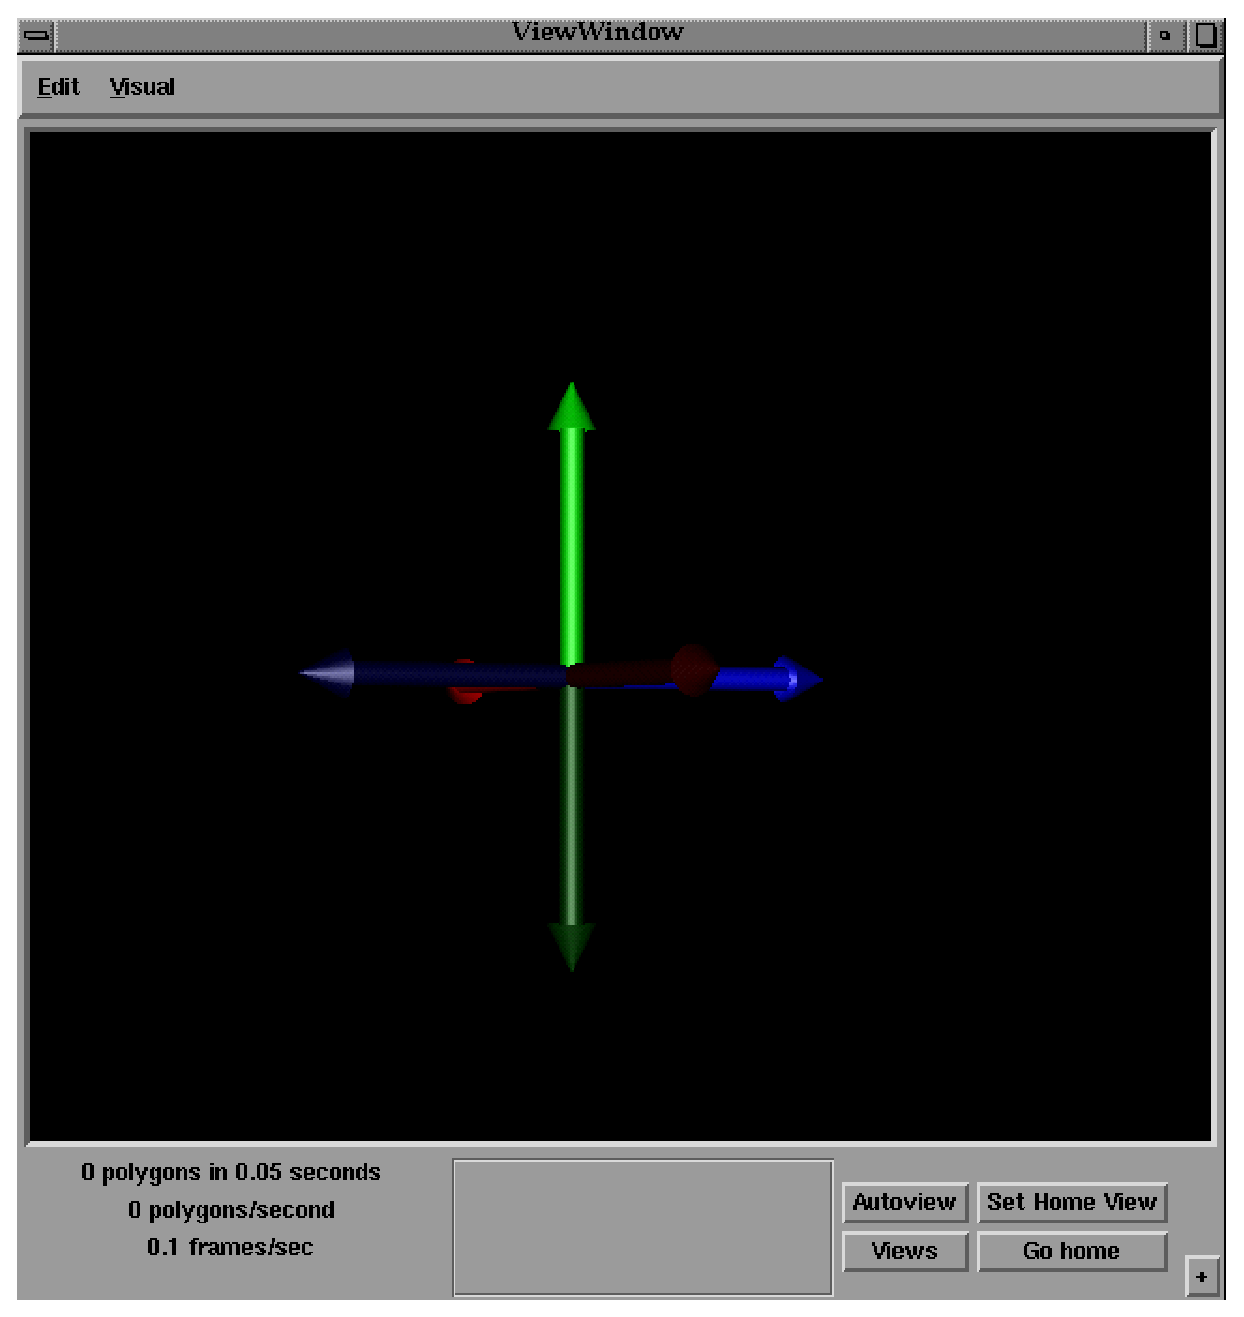
\epsfig{file=Figures/viewwindow.eps.gz,height=4in,
  bbllx=0, bblly=0, bburx=660, bbury=660}}}
%end{latexonly}
\begin{htmlonly}
  \newcommand{\viewerwindow}{%
  \htmladdimg[align=top,width=645,alt="module"]
  {../Figures/viewwindow.gif}}
\end{htmlonly}

%% View of the extended viewer window
%begin{latexonly}
  \newcommand{\extendedwindow}%
  {\centerline{\epsfig{file=Figures/viewbottom.eps.gz,height=4in,
  bbllx=0, bblly=0, bburx=654, bbury=293}}}
%end{latexonly}
\begin{htmlonly}
  \newcommand{\extendedwindow}{%
  \htmladdimg[align=top,width=649,alt="extended view window"]
  {../Figures/viewbottom.gif}}
\end{htmlonly}

%% Gauge widget image
%begin{latexonly}
  \newcommand{\gaugewidget}%
  {\centerline{\epsfig{file=Figures/widget-gauge.eps.gz,height=2in,
  bbllx=0, bblly=0, bburx=457, bbury=340}}}
%end{latexonly}
\begin{htmlonly}
  \newcommand{\gaugewidget}{%
  \htmladdimg[align=top,width=458,alt="gaugewidget"]
  {../Figures/widget-gauge.gif}}
\end{htmlonly}

%% Frame widget image
%begin{latexonly}
  \newcommand{\framewidget}%
  {\centerline{\epsfig{file=Figures/widget-frame.eps.gz,height=2in,
  bbllx=0, bblly=0, bburx=328, bbury=268}}}
%end{latexonly}
\begin{htmlonly}
  \newcommand{\framewidget}{%
  \htmladdimg[align=top,width=329,alt="framewidget"]
  {../Figures/widget-frame.gif}}
\end{htmlonly}

%% Box widget image
%begin{latexonly}
  \newcommand{\boxwidget}%
  {\centerline{\epsfig{file=Figures/widget-box.eps.gz,height=2in,
  bbllx=0, bblly=0, bburx=458, bbury=342}}}
%end{latexonly}
\begin{htmlonly}
  \newcommand{\boxwidget}{%
  \htmladdimg[align=top,width=459,alt="boxwidget"]
  {../Figures/widget-box.gif}}
\end{htmlonly}

%% Ring widget image
%begin{latexonly}
  \newcommand{\ringwidget}%
  {\centerline{\epsfig{file=Figures/widget-ring.eps.gz,height=2in,
  bbllx=0, bblly=0, bburx=507, bbury=467}}}
%end{latexonly}
\begin{htmlonly}
  \newcommand{\ringwidget}{%
  \htmladdimg[align=top,width=508,alt="ringwidget"]
  {../Figures/widget-ring.gif}}
\end{htmlonly}

%% Record movie dialog window
%begin{latexonly}
  \newcommand{\recordmoviewin}%
  {\centerline{\epsfig{file=Figures/record_movie_win.eps.gz,
  bbllx=0, bblly=0, bburx=257, bbury=175}}}
%end{latexonly}
\begin{htmlonly}
  \newcommand{\recordmoviewin}{%
  \htmladdimg[align=top,alt="Movie Recording Dialog"]
  {../Figures/record_movie_win.gif}}
\end{htmlonly}

%%%%%%%%%%%%%%%%%%%%%%%%%%%%%%%%%%%%%%%%%%%%%%%%%%%%%%%%%%%%%%%%%%%%%%
\newcommand{\graphics}{\emph{Graphics}}

\chapter{Visualization}
\label{ch:viewer}
\index{Viewer@\viewer{}}

This section describes the most frequently used \sr{} module,
the \viewer{}, which displays interactive graphical
output to the computer screen.  The \viewer{} is used any time the user
wants to see a geometry or spatial data. The \viewer{} also provides access to
many simulation parameters and controls, and indirectly initiates new
iterations of  simulation steps, which is important for computational steering (see \secref{Computational Steering}{sec:con-steering}).

This section begins with an overview of the \viewer{} window and its
controls, then describes the options and variations.

\section{Anatomy of the \viewer{} Window}
\label{sec:viewer-anatomy} 
\index{Viewer@\viewer{}!anatomy}

The \viewer{} window contains two main areas.  The upper portion,
which displays graphics and is called the \graphics{} window, and the
lower portion where the majority of control buttons are found.
Figure~\ref{fig:viewwindow} contains an example of a \viewer{} window.
In the \graphics{} window, viewing is controlled by the mouse, mouse
buttons, and various modifier keys (shift/control/alt).  In the lower
window there are several buttons and sliders. Their function is
described in this section.

\begin{figure}[htb]
  \begin{makeimage}
  \end{makeimage}
  \viewerwindow
%    \framebox{\parbox[3in]{\columnwidth}{The\dotfill Figure\\
%    \vspace{2in}\\
%    With some \dotfill dummy text}}
  \caption{\label{fig:viewwindow} The default \viewer{} window in \SR{}}
\end{figure}


The visible controls along the bottom of the \viewer{} window set default
configurations as follows:
%
\begin{description}
  \buttondesc{Autoview} Restores the display to a default
  condition.  Useful when some combination of settings result in
  objects disappearing from the view window.
  
  \buttondesc{Set Home View} Captures the setting of the current view
  so the user can return to it later by clicking the ``Go home''
  button.

  \buttondesc{Go home} Restores the current home view.
  
  \buttondesc{Views} Lists a number of standard viewing angles
  and orientations.  The view directions align with the Cartesian axes
  of the objects, and the ``Up vector'' option sets the orientation of
  the objects when viewed along the selected axis.
\end{description}

The display's rendering speed is shown in the lower left corner of the
\viewer{}'s control window.  

More controls can be revealed by clicking the
\latexhtml{\fbox{+}}{\button{[+]}} button in the lower right corner of
the \viewer{} window (see \secref{Extended Control Window}
{sec:view-control} for a description of extended controls).


\subsection{Menus}
\index{Viewer@\viewer{}!menus}

The \viewer{} window's menu bar contains the \menu{File}, \menu{Edit},
and \menu{Visual} menus.

\begin{description}
  \menudesc{File} The \menu{File} menu contains the following items:

  \begin{description}
    \menuitemdesc{Save Image...} Saves the contents of the \viewer{}
    window as an image to a file.  A dialog prompts the user for a
    file name, an image format, and an image size.
    
    \menuitemdesc{Record Movie...} Saves the contents of the \viewer{}
    window as a movie.  See \secref{Recording
      Movies}{sec:recordmovies} for more information.
  \end{description}
  
  % All of the items below need further explication.
  \menudesc{Edit} The \menu{Edit} menu contains the following items:
  \begin{description}
    \menuitemdesc{View/Camera...} Edit eye point, look
    at point, up vector, and field of view settings.

    \menuitemdesc{Light Sources...} Edit light sources,
    colors, and brightness.

    \menuitemdesc{Background...} Change the \viewer{}
    window's background color.

    \menuitemdesc{Clipping Planes...} Edit the orientation and visibility
    of clipping planes.

    \menuitemdesc{Point Size...} Increase or decrease the size of points.

    \menuitemdesc{Line Width...} Increase or decrease the width of lines.
    
    \menuitemdesc{Polygon Offset...} Set the polygon offset parameter.
    This parameter is used to improve rendering of coplanar
    polygons, lines, and points by offsetting polygons (by a small
    amount) from other objects.

    \menuitemdesc{Scene Materials...} Edit scene material properties.
  \end{description}

  \menudesc{Visual} Allows the user to select different
  graphics hardware settings that are available on the workstation.
  The list is ordered heuristically from most to least useful.
\end{description}

\section{Recording Movies}
\label{sec:recordmovies} 
\index{movies}

\begin{figure}[htb]
  \begin{makeimage}
  \end{makeimage}
  \recordmoviewin
  \caption{\label{fig:recordmoviewin} Movie Recording Window}
\end{figure}

The \viewer{}'s recording control window controls movie recording.  See
Figure~\ref{fig:recordmoviewin}.  Select \menuitem{Record Movie\dots} from
the \viewer{} window's \menu{File} menu to show the movie control window.

\sr{} records a movie by saving the content of the \viewer{} window to
a file each time the \viewer{} window is redrawn.

Two formats are supported, Silicon Graphic's RGB (``raw frames'') and
MPEG.

When recorded as raw frames, a movie will be saved as a series of RGB
files.  Each file is named as follows:
\filename{\replaceable{ddd}.\replaceable{name}.raw}, where
\replaceable{ddd} is a 3 digit frame number and \replaceable{name} is
the name typed into the control window's text entry field.

When recorded in the MPEG format all frames of a movie will be saved
in a file named \filename{\replaceable{name}.mpg}.

The width and height of each frame is the same size as the width and
height of the \viewer{} control window.  The width and height of each
frame may be changed by clicking button \guibutton{Resize} and typing
width and height values into the resize text boxes---this must be done
before recording the movie.

Click button \guibutton{Raw Frames} to begin a raw frames recording.
Click button \guibutton{Mpeg} to begin an MPEG recording.  Each new
\viewer{} window frame will be recorded.  Click button \guibutton{Stop
\ Recording} to end a movie.


\section{Mouse Control in the \viewer{} Window}
\label{sec:view-mouse} 
\index{Viewer@\viewer{}!mouse controls}

The \viewer{}'s mouse controls are extensive and flexible.  The
resulting action depends on the choice of mouse button, how the mouse
is moved and simultaneously pressed control keys.  The descriptions in
Tables~\ref{tab:view-mouse} and~\ref{tab:view-unicam} may seem
complicated, but with practice, use of the mouse becomes intuitive.


\begin{table}[htb]
\begin{center}
  \begin{tabular}{|l|l|p{5in}|} \hline
    \multicolumn{3}{|c|}{\large Mouse Controls}\\ \hline \hline 
    \multicolumn{1}{|c|}{Control Key} & 
    \multicolumn{1}{|c|}{Button} & 
    \multicolumn{1}{|c|}{Action}\\ \hline
None & Left & Translate scene \\
     & Middle & \begin{raggedleft} Rotate scene about its center on an arc
    ball that surrounds it; rotation direction is a function of the
    initial mouse location so try different sites and note the
    response. \end{raggedleft}\\  
     & Right & Zoom or scale scene (downwards and to the right increases
     size, upwards or to the left decreases size) \\ \hline
Shift & Left & Select and move a widget in the display \\
      & Middle & Toggle through the modes for a widget \\
      & Right & Pop up a widget information window \\ \hline
Control & Left & Translate in the Z-direction, \ie{} zoom in and out of the
    screen (down moves closer, up further away).  Moving left and
    right increases the ``throttle'' of the Z-direction motion.  If
    the cursor is over a point on an object when clicked, this point
    becomes the center of the screen for translation.\\ 
      & Middle & Rotate the camera view about the eye point (using arcball
    motion). \\ 
      & Right & Unicam movement (see Table~\ref{tab:view-unicam})\\ \hline
\end{tabular}
\caption{\label{tab:view-mouse} Mouse controls for the \viewer{}}
\end{center}
\end{table}

\bigskip

\begin{table}
\begin{center}
\begin{tabular}{|l|l|p{3in}|} \hline
    \multicolumn{3}{|c|}{\large Unicam movement (Control key and right mouse
    button} \\ \hline \hline
    \multicolumn{1}{|c|}{Initial mouse location} & 
    \multicolumn{1}{|c|}{Action} & \\ 
    \hline
    Near edge of display & Rotate objects on the arc ball & \\
    Near the objects & Following behavior: & \\
    \hline
    & \multicolumn{1}{|c|}{Initial mouse movement} & 
    \multicolumn{1}{|c|}{Action}\\ \hline
    & Horizontal & Pan objects \\ 
    & Vertical & Zoom and pan: down = zoom in, up = zoom
    out, left and right= pan left and right) \\
    & None & Set rotation point for subsequent arc ball rotation.\\
    \hline
\end{tabular}
\caption{\label{tab:view-unicam} Autocam mouse controls in the \viewer{}}
\end{center}
\end{table}



\section{Extended Control Window}
\label{sec:view-control} 
\index{Viewer@\viewer{}!extended controls}

Clicking on the \button{[+]} button in the lower right corner of the
default \viewer{} window expands to reveal an extended panel of
control buttons as shown in Figure~\ref{fig:extviewwindow}.  Note that
\button{[+]} changes to \button{[-]}.  Clicking on the \button{[-]}
button hides the extended control panel.  The following sections
describe the control options available in the extended control
window.

\begin{figure}[htb]
  \begin{makeimage}
  \end{makeimage}
  \extendedwindow
%    \framebox{\parbox[3in]{\columnwidth}{The\dotfill Figure\\
%    \vspace{2in}\\
%    With some \dotfill dummy text}}
  \caption{\label{fig:extviewwindow} The lower portion of extended
    \viewer{} window in \SR{}} 
\end{figure}


\subsection{Object Selector}

The lower portion of the extended \viewer{} window is divided into three
columns. The middle column contains a list of all objects in the
display.  If the list becomes long, use the scroll bar on the left
side to access other objects.  For each entry in the list there are
the following controls, reading from left to right:

\begin{itemize}
  \item At the left end of each object
        in the list is a selection indicator that displays red
        when that object is 
        selected.  The \viewer{} window only displays objects that
        are selected.
  \item Now comes the name of the object.
  \item Next the \button{Shading} control box determines the
        shading options used for rendering the object.
        Options include: Lighting, BBox, Fog, Use Clip, Back Cull, and
        Display List  (see
        \secref{Rendering controls}{sec:view-rendering} for directions).
  \item Lighting control is found at the right end of each entry, initially
        marked \menu{Default}.  In the Default setting, the common
        rendering controls described in \secref{Rendering
        controls}{sec:view-rendering} below apply.  Clicking this box
        reveals a set of options that only apply to this object that
        include Wire, Flat, and Gouraud.
\end{itemize}


\subsection{Rendering Controls}
\label{sec:view-rendering} 
\index{Viewer@\viewer{}!rendering}

The left column of the extended \viewer{} window contains controls that
apply to all selected objects with ``Default'' lighting selected.
Objects without the Default setting use their own object specific
settings, as described in the previous section.  

The lighting and shading options available are:
%
\begin{description}
  \descitem{Lighting} Toggles whether or not the \viewer{} applies
  lighting to the display.  Objects without lighting have a constant
  color.
        
  \descitem{Fog} Draws objects with variable intensity based on their
  distance from the user, also known as ``depth cueing''.  Close
  objects appear brighter while more remote objects fade gradually
  into the background as a function of distance from the front.
  
  \descitem{BBox} Toggles whether the \viewer{} draws the selected
  objects in full detail, or as a simple bounding box.
  
  \descitem{Use Clip} Applies up to six clipping planes to the
  display.  To control the clipping plane locations, use the ``Edit
  -\ra{} Clipping Planes'' menu at the top of the \viewer{} window.
  
  \descitem{Back Cull} Displays only the forward facing facets of any
  surface objects in the display.
  
  \descitem{Display List} Cache the list of objects to be displayed.
  This option accelerates rendering when the content of the display
  does not change.

  \descitem{Shading} Selects the type of shading for objects from the
        following options:
        \begin{description}
          \descitem{Wire} Show only the wire mesh of objects.
          \descitem{Flat} Draw each facet with a constant color.
          \descitem{Gouraud} Linearly interpolate the color across facets. 
        \end{description}
\end{description}

The right column of the extended \viewer{} window contains controls
for displaying the axes and creating stereoscopic rendering.  

\paragraph{Stereo viewing: } requires hardware LCD glasses synchronized
with the display, so visibility in each eye coincides with the
display of the appropriate view.  The ``Fusion Scale'' control provides a
means of setting the eye separation, and thus setting the view that is most
suited to facial anatomy and distance from the screen.

\section{Control Widgets}
\label{sec:view-widgets} 

\SR{} supports powerful display widgets.  Examples of widget
capabilities include managing cutting surfaces colored according to
the local data values, displaying streamlines in vector fields, or
selecting sub-volumes within the display area for further
manipulation.
 
\sci{} has made interaction with widgets as consistent as
possible. For example, controlling parameters is usually done by
clicking and dragging on a cylindrical ``collar'' or a sphere element
of the widget. Note that a single widget can have more than one
purpose depending on the context in which it exists. The Gauge widget,
for example, selects a clipping or display plane through a
three-dimensional object, and sets the seed points for a streamline
module.

This section describes the widgets available within \SR{} and \BIOPSE{}.
 
\subsection{Gauge Widget}
\label{sec:view-gaugewidget} 

\begin{figure}[htb]
  \begin{makeimage}
  \end{makeimage}
  \gaugewidget
%    \framebox{\parbox[3in]{\columnwidth}{The\dotfill Figure\\
%    \vspace{2in}\\
%    With some \dotfill dummy text}}
  \caption{\label{fig:gaugewidget} The gauge widget for setting location and
    density of seed points}
\end{figure}

\paragraph{Appearance} The Gauge
Widget has an orientation, length, and value (see Figure~\ref{fig:gaugewidget}). It consists of two spheres (A) connected by a cylinder (B) with a
small slider collar (C) on the cylinder.  There are also small resize
cylinders (D) extending from the spheres.

\paragraph{Purpose} The primary use of the Gauge Widget is to set the
location and density of streamlines emerging from the long cylinder.  It
can also be used as a more general purpose three-dimensional slider, or a
source for a stream surface. 

\paragraph{Controls} Clicking and dragging either sphere changes the widget's orientation.  Dragging either of the resize
cylinders causes the size of the widget to change, and dragging any point on
the main cylinder moves the whole widget without any change in orientation.
Dragging the slider collar changes the associated value, typically the
density of seed points for a streamline source.

\subsection{Frame Widget}
\label{sec:view-framewidget} 

\begin{figure}[htb]
  \begin{makeimage}
  \end{makeimage}
  \framewidget
%    \framebox{\parbox[3in]{\columnwidth}{The\dotfill Figure\\
%    \vspace{2in}\\
%    With some \dotfill dummy text}}
  \caption{\label{fig:framewidget} The Frame Widget}
\end{figure}


\paragraph{Appearance} The
Frame Widget (see Figure~\ref{fig:framewidget}) consists of four cylinders connected in a rectangle.  In
the middle of each cylinder there is a sphere (B), from which
a resize cylinder extends (C).

\paragraph{Purpose} The Frame Widget is primarily used for image
plane definition, defining stream volumes, and as a "tie dye'' similar to
the Ring Widget described in \secref{Ring Widget}{sec:view-ringwidget}.

\paragraph{Controls} Dragging a sphere rotates the widget about its center. Dragging on a resize cylinder extends or contracts the rectangle.
Dragging any cylinder drags the entire widget through space.


\subsection{Box Widget}
\label{sec:view-boxwidget} 

\begin{figure}[htb]
  \begin{makeimage}
  \end{makeimage}
  \boxwidget
%    \framebox{\parbox[3in]{\columnwidth}{The\dotfill Figure\\
%    \vspace{2in}\\
%    With some \dotfill dummy text}}
  \caption{\label{fig:boxwidget} The boxwidget for selecting sub-volumes}
\end{figure}

\paragraph{Appearance} The Box
Widget (see Figure~\ref{sec:view-boxwidget}) consists of twelve 
connected cylinders (A) to form a hexahedral box (B) (three-dimensional
rectangle).  In the middle of each face of the box is a sphere with a protruding cylinder (C) providing resize control.

\paragraph{Purpose} The Box Widget is primarily used to select a
subvolume of the workspace for further manipulation (\eg{} volume
rendering, isosurfaces, streamlines, mesh adaption) where the faces of the
widget act as orthogonal clipping planes.

\paragraph{Controls} Clicking on and dragging a sphere rotates
the widget about its center without changing the position of the center.
Clicking on and dragging any resize handle
% What do these look like??
causes the associated face to extend without changing its orientation.
Dragging a cylinder causes the entire widget to move without changing its
orientation.

\subsection{Ring Widget}
\label{sec:view-ringwidget} 

\begin{figure}[htb]
  \begin{makeimage}
  \end{makeimage}
  \ringwidget
%    \framebox{\parbox[3in]{\columnwidth}{The\dotfill Figure\\
%    \vspace{2in}\\
%    With some \dotfill dummy text}}
  \caption{\label{fig:ringwidget} The ring widget for selecting
    cutting/projection planes}
\end{figure}


\paragraph{Appearance} The Ring
Widget (see Figure~\ref{sec:view-ringwidget}) consists of a ring (A)
with four embedded spheres (B), each with a resize cylinder
attached (D).  Between two of the spheres is a sliding collar (C).
One of the resize cylinders has a special material property (typically
a different color from the other cylinders) to indicate that it is the
``halfway point'' for the slider (E).

\paragraph{Purpose} The Ring Widget is primarily used to set the
density of streamlines emerging from the ring. The ring serves as a set of
seed points from which streamlines emerge. The Ring Widget can 
serve as a three-dimensional angle gauge, as a source for multiple
streamlines throughout its surface, as a source for a stream surface from
the outer ring, and as a source for a stream volume.  The Ring Widget can 
also be used as a color sheet, or ``tie dye'', in which the surface is colored as 
a function of the scalar value of the field at each point.

\paragraph{Controls} Clicking and dragging the slider collar along the
ring changes the density of the seed points or some other related
parameter.  Dragging the spheres controls the orientation of the Ring
Widget, while moving the resize cylinders change the radius of the Ring
Widget about its center.  Dragging any other point on the ring moves the
ring in space without changing its radius or orientation.


%%% Local Variables: 
%%% mode: latex
%%% TeX-master: t
%%% End: 
